%08.03.2024
\section{Lecture 5}

continuation of unit 11

\subsection{Lower bounds for streaming algorithms}

We will start with basics on communication complexity.

\begin{df}[Communication Protocol?]
	Two players Alice and Bob. Alice knows string $x \in \{0, 1\}^n$ and Bob knows string $y \in \{0, 1\}^m$. And they can send one bit to each other. 
	
	The function $f \colon \{0, 1\}^n \times \{0, 1\}^m \to \{0, 1\}$ is given. They want to compute $f(x, y)$. Bob should know answer at the end of communication.
	
	They can send messages to each other. 
	We would take care of count of bits they sent and also count of rounds. By round we mean that first Alice sends some block of bits, after that Bob send something to Alice and so on.
\end{df}

We will get lower bounds on streaming algorithms through communication complexity.

\begin{remrk}
	Idea: Alice has $x$, Bob has $y$.
	In their mind they construct a stream with first half filled with $x$ and second part filled with $y$. After that they say: suppose there is an efficient algorithm for that stream. Then Alice will run this algorithm on first half of a stream(because Alice know $x$) and send memory of this algorithm to Bob. After that Bob just continue this algorithm on $y$.
	
	In our model it's a single round communication. If we can get lower bounds for $2k-1$-rounds protocol it would give us a lower bound on $2k$ passes streaming algorithm.
	Alice computes something on $x$, sends to Bob, Bob computes on $y$, sends to Alice and so on. See Fig. \ref{fig:streaming_to_communication}.


\begin{figure}[H]
\centering
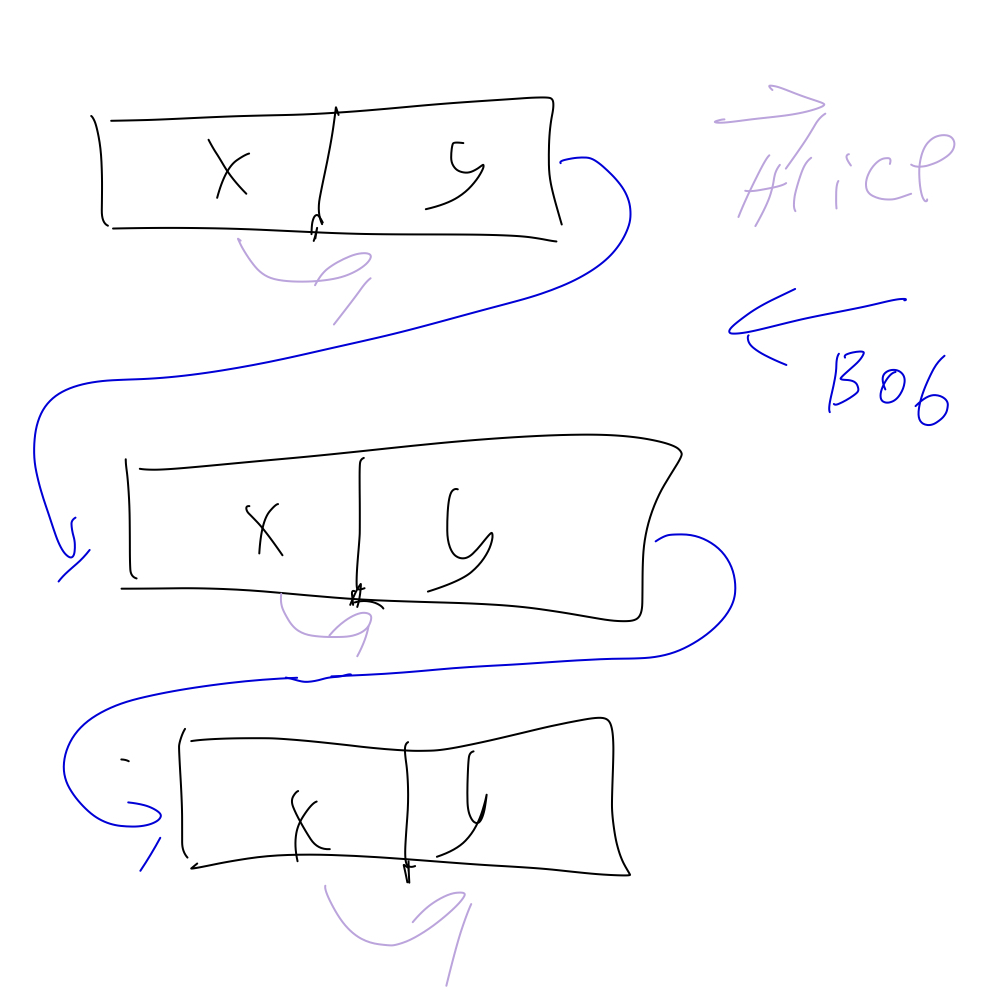
\includegraphics[width=0.4\linewidth]{figures/streaming_to_communication.jpeg}
\caption{From 5-rounds protocol to 3-passes streaming.}
\label{fig:streaming_to_communication}
\end{figure}
\end{remrk}

\begin{claim}
	If $C$ is a communication complexity for $2p - 1$ round protocol and $S$ is a space lower bound for $p$-passes streaming algorithm. Hence, using idea above we show that
	\begin{align*}
		C \leq (2p - 1) S \implies S \geq \frac C {2p - 1}
	\end{align*}
	
	And using this idea we cannot show a better lower bound.
\end{claim}

\begin{prop}
	We use notation $\cc(f)$ is a communication complexity of function $f$. 
\end{prop}

\begin{remrk}
	If we have rectangle $R = X \times Y$, where $X \subseteq \{0, 1\}^n$ and $Y \subseteq \{0, 1\}^m$, then if $R$ is a leaf(end of communication) then $R$ is monochromatic. Means that $\exists c \colon \forall (x, y) \in R \implies f(x, y) = c$.
\end{remrk}

\begin{remrk}
	Communication tree is a binary tree such that every node labeled with player who sends(Alice or Bob) and also if we look at rectangles of nodes. Then node splits rectangle either vertical or horizontal(based of player which sends message now).
	
	Can be proved easily by induction from the very bottom.
\end{remrk}


\begin{remrk}
To say that some function requires a lot of bits to be sent, we would should that in every communication tree count of leaves is huge. 
Easy to see that $L(f) \leq 2^{\cc(f)}$ where $L(f)$ denotes minimum amount of leaves in any communication tree for $f$. 
	
\end{remrk}

\begin{thm}[Equality problem]
	Given $n = m, \; \text{Eq}(x, y) = [x = y]$. We want to prove that $\cc(\text{Eq}) \geq n$.
\end{thm}

\begin{proof}
	It's easy to see that every monochromatic rectangle $(x, x)$ is of size 1 and two of them cannot be in the same bigger monochromatic rectangle. 
	Implies that $L(\text{Eq}) \geq 2^n \implies \cc(\text{Eq}) \geq n$.	
\end{proof}

\begin{thm}[Disjoint problem]
	Assume function:
	\begin{align*}
		\text{DISJ}(x, y) = \begin{cases}
			1, & \sum\limits_i x_i y_i = 0 \\
			0 & \text{otherwise}
		\end{cases}
	\end{align*}
	
	Then $\cc(\text{DISJ}) \geq n$.
\end{thm}

\begin{proof}
	Every monochromatic rectangle $(x, \overline x)$. Then, for every pair $(x, \overline x)$ and $(y, \overline y)$, then either $\text{DISJ}(x, \overline y) = 1$, either $\text{DISJ}(y, \overline x) = 1$, implies that $L(\text{DISJ}) \geq n$.
\end{proof}

\begin{thm}[Index problem]
	Assume function $\text{Index}(x, y) = x[y]$, where $x \in \{0, 1\}^{2^n}$ and $y \in [2^n]$.
	
	In one round model we have $\cc(\text{Index}) \geq 2^n$.
\end{thm}

\begin{proof}
	Otherwise some inputs for Alice would send same message. Implies that Bob can just set $y$ as a position of different bit in those Alice strings.
\end{proof}

\begin{lm}[Yao principal]
	\begin{align*}
		\max_\mu \cc_{\mu, \eps}(f) = R_\eps(f)
	\end{align*}, where $R_\eps$ is a randomized complexity with a probability of error at most $\eps$. Alice and Bob gets same random string $r$ and they output $f(x, y)$ with probability of success at least $1 - \eps$.
	
	And $\mu$ in $CC_{\mu, \eps}(f)$ is some distribution over inputs($(x, y) \sim \mu$) and we need to solve a problem deterministically assuming that inputs are distributed with $\mu$.
\end{lm}

\begin{proof}
	Let's define a game. Player I choose a deterministic algorithm and player II choose an input. Player I wins if algorithm outputs correct output, II wins otherwise.
	
	Let's take a look on randomized protocol from $R_\eps(f)$, distribution over random bits $r$ of that protocol gives us correct distribution $\sigma$ over deterministic protocols. So there is a bijection between distribution on protocols and randomized protocol. Hence, there exists $\sigma$ ~-- distribution over protocols of depth $\leq R_\eps(f)$ such that for every input $(x, y)$ probability 
	\begin{align*}
		\Pr_{P \sim \sigma} [P(x, y) = f(x, y)] \geq 1 - \varepsilon
	\end{align*}, where $P$ is a deterministic protocol for $f$ of depth $\leq R_\eps(f)$.
	
	
 	Now using Nash Theorem we get that there exists a mixed strategy with Nash equilibrium. Moreover, it says that $\max_I \min_{II} = \min_{II} \max_I$ and that we can use mixed strategy for first player and pure for second(and vice versa).
	Assume that all protocols have bounded depth $t$.
	
	\begin{align*}
		\max_\sigma \min_\chi \Pr_{\substack{P \sim \sigma \\ (x, y) \sim \chi}}[P(x, y) = f(x, y)] &= \min_\chi \max_\sigma \Pr_{\substack{P \sim \sigma \\ (x, y) \sim \chi}}[P(x, y) = f(x, y)] \\
		\max_\sigma \min_{(x, y)} \Pr_{P \sim \sigma}[P(x, y) = f(x, y)] &= \min_\chi \max_{P} \Pr_{(x, y) \sim \chi}[P(x, y) = f(x, y)]
	\end{align*}
	
	Assume that this $\max \min$ equals to $1 - \eps_t$.
	
	Then $R_\eps(f) = \min \{t \mid \eps_t \leq \eps \}$, using left part of last equality.
	
	And we can see that $\max_\mu \cc_{\mu, \eps}(f) = \min \{t \mid \eps_t \leq \eps\}$ using right part of last equality.
	
	Which finished our proof.
\end{proof}

Typically we would use this theorem in form that $R_\eps(f) \geq \max_\mu \cc_{\mu, \eps}(f)$.

\begin{df}[INX - Randomized Index problem] \label{problem:INX}
	Let $\eps$ be a probability of error. $f(x, y) = x[y]$, where $x \in \{0, 1\}^{2^n}, y \in 2^n$.
	Complexity of this problem is $R_\eps(f)$.
\end{df}

\begin{thm}
	Let $x \sim_U \{0, 1\}^{2^n}$ and $y \sim_U [2^n]$(i.e. $\chi$ is a uniform distribution).	
	Then,~$\cc_{U, \eps} \geq 2^{\alpha n}$ for one round protocol.
\end{thm}

\begin{proof}
	Suppose for some protocol $P$ satisfies
	\begin{align*}
		\Pr_{(x, y)\sim U}[P(x, y) \neq x_y] \leq \frac 1 {20}
	\end{align*}
	
	Then
	\begin{align*}
		\E_x[\Pr_y[P(x, y) \neq x_y]] \leq \frac 1 {20} &\implies \\
&\Pr_x\left[\Pr_y[P(x, y) \neq x_y] \geq \frac 2 {20}\right] \leq \frac 1 2
	\end{align*} By Markov's inequality.
	
	Implies that there is a set $S$ such that $|S| \geq \dfrac {2^n} 2$ such that
	\begin{align*}
		\forall x \in S \implies \Pr_y[P(x, y) \neq x_y] \leq \frac 1 {10}
	\end{align*}
	
	The idea is take those inputs from $S$ and look only on them.
	Our output should be correct almost all times, so Bob should identify what Alice has sent to him.
	
	From now on $x \in S$, so Bob has some function $g(m(x), y) = P(x, y)$, where $m(x)$ is a message that Alice send to Bob on input $x$.
	Let $w(m) = [g(m, 1), g(m, 2), \dots, g(m, 2^n)]$, then avarage distance $\E H(x, w(m(x))) \leq 2^n \cdot \dfrac 1 {10} = \dfrac {2^n} {10}$.
	
	Let $x_1, x_2 \in S$ such that $m(x_1) = m(x_2)$ and let $w(m(x_1)) = w(m(x_2) ) = y$, then using triangle inequality we have that $H(x_1, x_2) \leq H(x_1, y) + H(x_2, y) \leq \dfrac 1 5 2^n$.
	
	The well known fact that there exists such $S_2 \subseteq S \colon \forall x_1, x_2 \in S_2 \implies H(x_1, x_2) > \dfrac {2^n} 5$ and $|S_2| \geq 2^{\alpha n}$ for some $\alpha > 0$, then message for any two elements of $S_2$ should be different.
	
	To construct such $S_2$ we take random subset of $\{0, 1\}^n$ of proper size, says that with high probability it's satisfies our conditions and with high probability a lot of elements from $S$ are in $S_2$.
	
	Implies that $\cc_{U, \eps} (f) \geq 2^{\alpha n}$.
\end{proof}

\begin{crly}
	$R_\eps \geq 2^{\alpha n}$ for INX \ref{problem:INX} problem in terms of one round protocols.
\end{crly}
\begin{proof}
		We know that $\cc_{U, \eps} \geq 2^{\alpha n}$, it's implies that $\max_\mu CC_{\mu, \eps} \geq 2^{\alpha n}$, hence $R_\eps \geq 2^{\alpha n}$ for some $\alpha > 0$.
\end{proof}


